\documentclass{article}

\usepackage[utf8]{inputenc}
\usepackage{fullpage}
\usepackage{amsmath, amssymb, amsfonts, amsthm}
\usepackage{bbm}
\usepackage{mathtools}
\usepackage{twoopt}
\usepackage{babel}
\usepackage{tikz}
\usepackage{enumitem}

\def \lastexercisenumber {0}

% special letters:

\newcommand{\N}{\mathbb{N}}
\newcommand{\Z}{\mathbb{Z}}
\newcommand{\Q}{\mathbb{Q}}
\newcommand{\R}{\mathbb{R}}
\newcommand{\C}{\mathbb{C}}
\newcommand{\K}{\mathbb{K}}
\newcommand{\T}{\mathbb{T}}
\newcommand{\E}{\mathbb{E}}
\newcommand{\V}{\mathbb{V}}
\renewcommand{\S}{\mathbb{S}}
\renewcommand{\P}{\mathbb{P}}
\newcommand{\1}{\mathbbm{1}}

% quantors:

\newcommand{\Forall}{\forall \,}
\newcommand{\Exists}{\exists \,}
\newcommand{\ExistsOnlyOne}{\exists! \,}
\newcommand{\nExists}{\nexists \,}
\newcommand{\ForAlmostAll}{\forall^\infty \,}

% MISC symbols:

\newcommand{\landau}{{\scriptstyle \mathcal{O}}}
\newcommand{\Landau}{\mathcal{O}}


\newcommand{\eps}{\mathrm{eps}}

% graphics in a box:

\newcommandtwoopt
{\includegraphicsboxed}[3][][]
{
  \begin{figure}[!h]
    \begin{boxedin}
      \ifthenelse{\isempty{#1}}
      {
        \begin{center}
          \includegraphics[width = 0.75 \textwidth]{#3}
          \label{fig:#2}
        \end{center}
      }{
        \begin{center}
          \includegraphics[width = 0.75 \textwidth]{#3}
          \caption{#1}
          \label{fig:#2}
        \end{center}
      }
    \end{boxedin}
  \end{figure}
}

% braces:

\newcommand{\pbraces}[1]{{\left  ( #1 \right  )}}
\newcommand{\bbraces}[1]{{\left  [ #1 \right  ]}}
\newcommand{\Bbraces}[1]{{\left \{ #1 \right \}}}
\newcommand{\vbraces}[1]{{\left  | #1 \right  |}}
\newcommand{\Vbraces}[1]{{\left \| #1 \right \|}}
\newcommand{\abraces}[1]{{\left \langle #1 \right \rangle}}
\newcommand{\round}[1]{\bbraces{#1}}

\newcommand
{\floorbraces}[1]
{{\left \lfloor #1 \right \rfloor}}

\newcommand
{\ceilbraces} [1]
{{\left \lceil  #1 \right \rceil }}

% special functions:

\newcommand{\norm}  [2][]{\Vbraces{#2}_{#1}}
\newcommand{\diam}  [2][]{\mathrm{diam}_{#1} \: #2}
\newcommand{\diag}  [1]{\mathrm{diag} \: #1}
\newcommand{\dist}  [1]{\mathrm{dist} \: #1}
\newcommand{\mean}  [1]{\mathrm{mean} \: #1}
\newcommand{\erf}   [1]{\mathrm{erf} \: #1}
\newcommand{\id}    [1]{\mathrm{id} \: #1}
\newcommand{\sgn}   [1]{\mathrm{sgn} \: #1}
\newcommand{\supp}  [1]{\mathrm{supp} \: #1}
\newcommand{\arsinh}[1]{\mathrm{arsinh} \: #1}
\newcommand{\arcosh}[1]{\mathrm{arcosh} \: #1}
\newcommand{\artanh}[1]{\mathrm{artanh} \: #1}
\newcommand{\card}  [1]{\mathrm{card} \: #1}
\newcommand{\Span}  [1]{\mathrm{span} \: #1}
\newcommand{\Aut}   [1]{\mathrm{Aut} \: #1}
\newcommand{\End}   [1]{\mathrm{End} \: #1}
\newcommand{\ggT}   [1]{\mathrm{ggT} \: #1}
\newcommand{\kgV}   [1]{\mathrm{kgV} \: #1}
\newcommand{\ord}   [1]{\mathrm{ord} \: #1}
\newcommand{\grad}  [1]{\mathrm{grad} \: #1}
\newcommand{\ran}   [1]{\mathrm{ran} \: #1}
\newcommand{\graph} [1]{\mathrm{graph} \: #1}
\newcommand{\Inv}   [1]{\mathrm{Inv} \: #1}
\newcommand{\pv}    [1]{\mathrm{pv} \: #1}
\newcommand{\GL}    [1]{\mathrm{GL} \: #1}
\newcommand{\Mod}{\mathrm{Mod} \:}
\newcommand{\Th}{\mathrm{Th} \:}
\newcommand{\Char}{\mathrm{char}}
\newcommand{\At}{\mathrm{At}}
\newcommand{\Ob}{\mathrm{Ob}}
\newcommand{\Hom}{\mathrm{Hom}}
\newcommand{\orthogonal}[3][]{#2 ~\bot_{#1}~ #3}
\newcommand{\Rang}{\mathrm{Rang}}
\newcommand{\NIL}{\mathrm{NIL}}
\newcommand{\Res}{\mathrm{Res}}
\newcommand{\lxor}{\dot \lor}
\newcommand{\Div}{\mathrm{div} \:}
\newcommand{\meas}{\mathrm{meas} \:}

% fractions:

\newcommand{\Frac}[2]{\frac{1}{#1} \pbraces{#2}}
\newcommand{\nfrac}[2]{\nicefrac{#1}{#2}}

% derivatives & integrals:

\newcommandtwoopt
{\Int}[4][][]
{\int_{#1}^{#2} #3 ~\mathrm{d} #4}

\newcommandtwoopt
{\derivative}[3][][]
{
  \frac
  {\mathrm{d}^{#1} #2}
  {\mathrm{d} #3^{#1}}
}

\newcommandtwoopt
{\pderivative}[3][][]
{
  \frac
  {\partial^{#1} #2}
  {\partial #3^{#1}}
}

\newcommand
{\primeprime}
{{\prime \prime}}

\newcommand
{\primeprimeprime}
{{\prime \prime \prime}}

% Text:

\newcommand{\Quote}[1]{\glqq #1\grqq{}}
\newcommand{\Text}[1]{{\text{#1}}}
\newcommand{\fastueberall}{\text{f.ü.}}
\newcommand{\fastsicher}{\text{f.s.}}

% -------------------------------- %
% amsthm-stuff:

\theoremstyle{definition}

% numbered theorems
\newtheorem{theorem}{Satz}
\newtheorem{lemma}{Lemma}
\newtheorem{corollary}{Korollar}
\newtheorem{proposition}{Proposition}
\newtheorem{remark}{Bemerkung}
\newtheorem{definition}{Definition}
\newtheorem{example}{Beispiel}

% unnumbered theorems
\newtheorem*{theorem*}{Satz}
\newtheorem*{lemma*}{Lemma}
\newtheorem*{corollary*}{Korollar}
\newtheorem*{proposition*}{Proposition}
\newtheorem*{remark*}{Bemerkung}
\newtheorem*{definition*}{Definition}
\newtheorem*{example*}{Beispiel}

% Please define this stuff in project ("main.tex"):

% \def \lastexercisenumber {...}
% This will be 0 by default

% \setcounter{section}{...}
% This will be 0 by default
% and hence, completely ignored

\ifnum \thesection = 0
{\newtheorem{exercise}{Aufgabe}}
\else
{\newtheorem{exercise}{Aufgabe}[section]}
\fi

\ifdef
{\lastexercisenumber}
{\setcounter{exercise}{\lastexercisenumber}}

\newcommand{\solution}
{
    \renewcommand{\proofname}{Lösung}
    \renewcommand{\qedsymbol}{}
    \proof
}

\renewcommand{\proofname}{Beweis}

% -------------------------------- %
% environment zum einkasteln:

% dickere vertical lines
\newcolumntype
{x}
[1]
{!{\centering\arraybackslash\vrule width #1}}

% environment selbst (the big cheese)
\newenvironment
{boxedin}
{
  \begin{tabular}
  {
    x{1 pt}
    p{\textwidth}
    x{1 pt}
  }
  \Xhline
  {2 \arrayrulewidth}
}
{
  \\
  \Xhline{2 \arrayrulewidth}
  \end{tabular}
}

% -------------------------------- %
% MISC "Ein-Deutschungen"

\renewcommand
{\figurename}
{Abbildung}

\renewcommand
{\tablename}
{Tabelle}

% -------------------------------- %


\parindent 0pt

\title
{
  Differentialgleichungen 1 - Übung 1 \\
  \vspace{4pt}
  \normalsize
  \textit{1. UE am 12.03.2020}
}
\author
{
  Richard Weiss       \and
  Florian Schager     \and
  Christian Sallinger \and
  Fabian Zehetgruber  \and
  Paul Winkler        \and
  Christian Göth
}
\date{}

\begin{document}

\maketitle

\begin{exercise}

Geben Sie bei den folgenden 4 Differentialgleichungen die Ordnung an und ob sie linear (oder nichtlinear)
sind.

\begin{enumerate}[label = \textbf{\alph*)}]
  \item $y^\prime(t) + y(t) \sin(t)  = 1,$
  \item $y^\primeprime(t)  = t \sin(y(t))$
  \item $\frac{\partial^2}{\partial x^2} u(x, y) + \frac{\partial^2}{\partial y^2} u(x, y)  = 0,$
  \item $\mathbf{y}^\prime(t) + \mathbf{A}(t) \mathbf{B}(t) \mathbf{y}(t)  = \mathbf{f}(t)$
\end{enumerate}

wobei $y: \R \to \R$, $u: R^2 \to R$, $y: \R \to \R^2$, $f \in C(\R; \R^2)$, $A, B \in C(\R; \R^{2 \times 2})$.

\end{exercise}

\begin{solution}

Trivial! (Diesmal wirklich)

\begin{enumerate}[label = \textbf{\alph*)}]
  \item Ordnung: 1 + linear
  \item Ordnung: 2 + nichtlinear
  \item Ordnung: 2 + partiell + linear
  \item Ordnung: 1 + linear
\end{enumerate}

\end{solution}

\begin{exercise}

Überführen Sie die folgenden skalaren Gleichungen 2. Ordnung in Systeme 1. Ordnung:

\begin{enumerate}[label = \textbf{\alph*)}]

  \item $y^\primeprime(t) + \sin(y^\prime(y^\prime(t))) = y(t)$

  \item $y^\primeprime(t) = -y(t) \cos(t)$

\end{enumerate}

Ist das Umschreiben in ein System 1. Ordnung eindeutig?

\end{exercise}

\begin{solution}

Trivial!

\begin{enumerate}[label = \textbf{\alph*)}]

  \item
  \begin{align*}
    y_1(t) & = y^\prime(t) \\
    y_1^\prime(t) & = y(t) - \sin(y_1(y_1(t)))
  \end{align*}

  \item
  \begin{align*}
    y_1(t) & = y^\prime(t) \\
    y_1^\prime(t) & = -y(t)\cos(t)
  \end{align*}

\end{enumerate}

Das Umschreiben ist im Allgemeinen nicht eindeutig.
Die Variablen können grundsätzlich beliebig gewählt werden (z.B. Vielfache).

\end{solution}

\begin{exercise}

Betrachten Sie die \textit{autonome}, explizite Differentialgleichung $y^{(k)}(t) = f(y(t), y^\prime(t), \ldots, y^{(k-1)}(t))$.
Sei $t_0 \in \R$.
Zeigen Sie:
Falls $y$ eine Lösung der ODE ist, dann ist auch $\phi: t \mapsto y(t - t_0)$ eine Lösung.

\end{exercise}

\begin{solution}

Damit die Aufgabe lösbar ist, müssen wir zusätzlich annehmen, dass das nicht angegebene offene Intervall $J = \R$.
Außerdem verlangen wir $f: G \mapsto \R^n$ mit dem Gebiet $G := \R^{n \times k}$. \\

$y$ ist eine Lösung der obigen ODE, falls

\begin{enumerate}[label = (\roman*)]

  \item $y \in C^k(J;\mathbb{R}^n)$,

  \item $\text{graph~} y := \{(y(t), y^\prime(t), \ldots, y^{(k-1)}(t)): t \in J\} \subset G$, und

  \item $\forall t \in J: y^{(k)}(t) = f(y(t), y^\prime(t), \ldots, y^{(k-1)}(t))$.

\end{enumerate}

Das soll nun auch für $\phi$ gelten:

\begin{enumerate}[label = (\roman*)]

  \item
  Da $y \in C^k(\R; \R^n)$ ist, aufgrund der Kettenregel, auch $\phi = y \circ \tau_{-t_0} \in C^k(\R; \R^n)$.

  \item
  Nachdem wir annehmen, dass $G = \R^{n \times k}$, ist auch die zweite Bedingung für $\phi$ erfüllt.

  \item
  Schließlich folgt, mit der Kettenregel, auch die dritte Bedingung, also $\Forall t \in J:$
  \begin{align*}
    \phi^{(k)}(t)
    =
    y^{(k)}(t-t_0)
    =
    f(y(t- t_0), y^\prime(t - t_0), \ldots, y^{(k-1)}(t-t_0))
    =
    f(\phi(t), \phi^\prime(t), \ldots, \phi^{(k-1)}(t)).
  \end{align*}

\end{enumerate}


\end{solution}

\begin{exercise}

Sei $\mathbf{A} \in C(\R; \R^{d \times d})$. Betrachten Sie die Differentialgleichung

\begin{align*}
  \mathbf{y}^\prime(t) + \mathbf{A}(t) \mathbf{y}(t) = 0 \in \R^d.
\end{align*}

Zeigen Sie: Die Menge aller Lösungen (genauer: zu gegebenem offenen Intervall $I \subset \R$ die Menge der $C^1(I; \R^d)$-Funktionen, die die Differentialgleichung erfüllen) ist ein Vektorraum.

\end{exercise}

\begin{solution}

\begin{align*}
  V := \pbraces{\R^d}^I,
  \quad
  U := \Bbraces
  {
    \mathbf{y} \in C^1(I; \R^d):
    \mathbf{y}^\prime + \mathbf{A} \mathbf{y} = 0
  }
\end{align*}

Wir zeigen, dass $U$ ein linearer Unterraum des Vektorraumes $V$ über $\R$ ist.

\begin{itemize}

  \item $0 \in U
  \Rightarrow
  U \neq \emptyset$

  \item $\Forall \mathbf{y}_1, \mathbf{y}_2 \in U, \Forall x \in \R:$
  \begin{align*}
    (\mathbf{y}_1 + x \mathbf{y}_2)^\prime +
    \mathbf{A}
    (\mathbf{y}_1 + x \mathbf{y}_2)
    =
    \underbrace{\pbraces{
      \mathbf{y}_1^\prime + \mathbf{A} \mathbf{y}_1
    }}_0 +
    x
    \underbrace{\pbraces{
    \mathbf{y}_2^\prime + \mathbf{A} \mathbf{y}_2
    }}_0
    = 0 \\
    \Rightarrow \mathbf{y}_1 + x \mathbf{y}_2 \in U
  \end{align*}

\end{itemize}

\end{solution}

\begin{exercise}

Sei $\epsilon > 0$. Betrachten Sie die \Quote{skalierte} Lotka-Volterra Gleichung

\begin{align*}
  x^\prime(t) & = x(t) - x(t) y(t) \\
  y^\prime(t) & = -\epsilon y(t) + x(t) y(t).
\end{align*}

Zeigen Sie: Die Funktion $(x, y) \mapsto \phi(x, y) := x + y - \epsilon \ln{x} - \ln{y}$ ist eine Erhaltungsgröße, d.h. für Lösungen $t \mapsto (x(t), y(t))$ der Lotka-Volterra-Gleichung gilt, daß $t \mapsto \phi(x(t), y(t))$ konstant ist.

\end{exercise}

\begin{solution}

Die Ableitung der Funktion $f: t \mapsto \phi(x(t), y(t))$ verschwindet.

\begin{align*}
  f^\prime(t)
  & =
  x^\prime(t) +
  y^\prime(t) -
  \epsilon
  \frac{1}{x(t)} x^\prime(t) -
  \frac{1}{y(t)} y^\prime(t) \\
  & =
  x(t) - x(t) y(t) -
  \epsilon
  y(t) + x(t) y(t) -
  \epsilon
  \frac{1}{x(t)}
  \pbraces
  {
    x(t) - x(t) y(t)
  } -
  \frac{1}{y(t)}
  \pbraces
  {
    -\epsilon
    y(t) + x(t) y(t)
  } \\
  & =
  x(t) - \epsilon y(t) - \epsilon + \epsilon y(t) + \epsilon - x(t) = 0
\end{align*}

\end{solution}

\begin{exercise}

Das \Quote{mathematische Pendel} wird beschrieben durch die ODE
\begin{align*}
  \varphi^\primeprime(t) + \omega^2 \sin{\varphi(t)} = 0,
  \quad
  \omega = \frac{g}{\ell},
\end{align*}

wobei $g$ die Erdbeschleunigung und $\ell$ die Fadenlänge des Pendels ist. Die Funktion $\varphi: t \mapsto \varphi(t)$ beschreibt die Auslenkung des Pendels.

\begin{enumerate}[label = \textbf{\alph*)}]

  \item Schreiben Sie die ODE in ein System 1. Ordnung um. Hat Ihre neue Variable eine physikalische
  Bedeutung?

  \item Geben Sie eine Erhaltungsgröße an. Begründen Sie, warum es sich um solche handelt.

\end{enumerate}

\end{exercise}

\begin{solution}

(a)

\begin{align*}
  \psi(t) & := \varphi^\prime(t) \\
  \psi^\prime(t) + \omega^2 \sin{\varphi(t)} & = 0
\end{align*}

$\psi$ ist die Winkelgeschwindigkeit des Pendels.

\begin{figure}[h!]
  \centering
  \begin{figure}
\centering

\begin{tikzpicture}



\end{tikzpicture}

\caption{title}
\end{figure}

  \caption{Pendel}
\end{figure}

(b) Die Energie ist eine Erhaltungsgröße. Um das nachzuweisen, stellen wir folgendes Modell auf.

\begin{itemize}
  \item
  $E(t) := E_\Text{pot}(t) + E_\Text{kin}(t)
  \ldots \text{Energie des Pendels}$
  \item
  $E_\Text{pot} := m \cdot g \cdot h(t)
  \ldots \text{potentielle Energie des Pendels}$
  \item
  $E_\Text{kin} := \Frac{2}{m \cdot v(t)^2}
  \ldots \text{kinetische Energie des Pendels}$
  \item
  $m \in \R^+
  \ldots \text{Masse des Pendels}$
  \item
  $h(t) := \ell - \ell \cdot \cos{\varphi(t)} + h_0
  \ldots \text{Höhe des Pendels}$
  \item
  $h_0 \in \R^+
  \ldots \text{Höhe des Pendels im Ruhezustand (d.h. minimale Höhe)}$
  \item
  $v(t) := \psi(t) \cdot \ell
  \ldots \text{Tangentialgeschwindigkeit des Pendels}$
\end{itemize}

Die Ableitung der Funktion $E$ verschwindet.

\begin{multline*}
  E^\prime(t)
  =
  E_\Text{pot}^\prime(t) + E_\Text{kin}^\prime(t)
  =
  m g h^\prime(t) + \Frac{2}{m \pbraces{v(t)^2}^\prime}
  =
  m g \ell \sin{\varphi(t) \varphi^\prime(t)} +
  \Frac{2}{2 m v(t) v^\prime(t)} \\
  =
  m g \ell \sin{\varphi(t) \varphi^\prime(t)} +
  m \varphi^\prime(t) \ell \varphi^\primeprime(t) \ell
  =
  m g \ell \sin{\varphi(t) \varphi^\prime(t)} -
  m \varphi^\prime(t) \ell \frac{g}{\ell} \sin{\varphi(t)} \ell = 0
\end{multline*}

\end{solution}

\begin{exercise}

Die Gleichung

\begin{align*}
  \frac{x^2}{a^2} + \frac{y^2}{b^2} = 1
\end{align*}

beschreibt eine Ellipse in der Ebene.
Zeichnen Sie die Ellipse.
Bestimmen Sie einen Tangentialvektor, einen Normalvektor und die Gleichung der Tangente an die Ellipse in einem beliebigen Punkt $(x_0, y_0)$ der Ellipse.
Machen Sie dies auf zwei Arten:

\begin{enumerate}[label = \textbf{\alph*)}]

  \item durch Auflösen der Gleichung nach $x$ oder $y$.

  \item unter Verwendung der Parametrisierung
  \begin{align*}
    x(t) = a \cos{t},
    \quad
    y(t) = b \sin{t},
    \quad
    t \in [0, 2 \pi].
  \end{align*}

\end{enumerate}

\end{exercise}

\begin{solution}

Die Ellipse $E$ ist also

\begin{align*}
  E :=
  \Bbraces
  {
    (x, y) \in \R^2:
    \frac{x^2}{a^2} + \frac{y^2}{b^2} = 1
  }
\end{align*}

und sieht wie folgt aus.

\begin{figure}[h!]
  \centering
  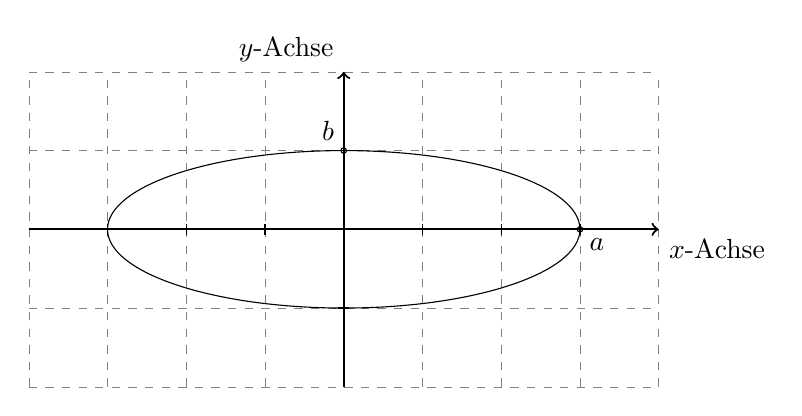
\begin{tikzpicture}

\draw
[step = 1cm, gray, very thin, dashed]
(-4, -2) grid (4, 2);

\draw
[thick, ->]
(-4, 0) -- (4, 0)
node[anchor = north west]{$x$-Achse};

\draw
[thick, ->]
(0, -2) -- (0, 2)
node[anchor = south east]{$y$-Achse};

\foreach \x in {-3, -2, -1, 0, 1, 2, 3}
  \draw (\x cm, 2pt) -- (\x cm, -2pt);

\foreach \y in {-1, 0, 1}
  \draw (2pt, \y cm) -- (-2pt, \y cm);

\draw (0, 0) ellipse (3cm and 1cm);

\draw
(3, 0) circle (1pt)
node[anchor = north west]{$a$};

\draw
(0, 1) circle (1pt)
node[anchor = south east]{$b$};

\end{tikzpicture}

  \caption{Ellipse}
\end{figure}

(a) Wir lösen die Gleichung nach $y$ auf und erhalten

\begin{align*}
  y_\pm = \pm b \sqrt{1 - \pbraces{\frac{x}{a}}^2}.
\end{align*}

Fasst man das als Funktion von $x$ auf so ergibt sich für die Ableitung

\begin{align*}
  y^\prime_{\pm}(x)
  =
  \mp \frac{2bx}{a^2 \sqrt{1 - \pbraces{\frac{x}{a}}^2}}.
\end{align*}

Ein Tangentialvektor $\vec{t}(x_0, y_0)$ im Punkt $(x_0, y_0)^T \in E$ der Ellipse ist

\begin{align*}
  \vec{t}(x_0, y_0)
  =
  \begin{cases}
    (1, y_+^\prime(x_0))^T,
    & \text{wenn} \enspace y_0 > 0, \\
    (0, 1)^T,
    & \text{wenn} \enspace y_0 = 0, \\
    (1, y_-^\prime(x_0))^T,
    & \text{wenn} \enspace y_0 < 0.
  \end{cases}
\end{align*}

Ein Normalvektor $\vec{n}(x_0, y_0)$ im Punkt $(x_0, y_0)^T \in E$ der Ellipse ist

\begin{align*}
  \vec{n}(x_0, y_0)
  =
  \begin{cases}
    (-y_+^\prime(x_0), 1)^T
    & \text{wenn} \enspace y_0 > 0, \\
    (1, 0)^T
    & \text{wenn} \enspace y_0 = 0, \\
    (-y_-^\prime(x_0), 1)^T
    & \text{wenn} \enspace y_0 < 0.
  \end{cases}
\end{align*}

Die Tangentengleichung $\vec{T}(x_0, y_0)$ im Punkt $(x_0, y_0)^T \in E$ der Ellipse ist

\begin{align*}
  \vec{T}(x_0, y_0)
  =
  \Bbraces
  {
    (x, y) \in \R^2:
    \begin{cases}
      y = y_0 + (x - x_0)y_+^\prime(x_0)
      & \text{wenn} \enspace y_0 > 0 \\
      x = \pm a
      & \text{wenn} \enspace y_0 = 0 \land x_0 = \pm a \\
      y = y_0 + (x - x_0) y_-^\prime(x_0)
      & \text{wenn} \enspace y_0 < 0
    \end{cases}
  }.
\end{align*}

(b) Nun parametrisieren wir die Ellipse gemäß Angabe. Ein Tangentialvektor $\vec{t}(t)$ in Abhängigkeit von $t$ ist

\begin{align*}
  \vec{t}(t)
  =
  \begin{pmatrix}
    x^\prime(t) \\ y^\prime(t)
  \end{pmatrix}
  =
  \begin{pmatrix}
    -a \sin(t) \\ b \cos(t)
  \end{pmatrix}.
\end{align*}

Ein Normalvektor $\vec{n}(t)$ in Abhängigkeit von $t$ ist

\begin{align*}
  n(t)
  =
  \begin{pmatrix}
    b \cos(t) \\ a \sin(t)
  \end{pmatrix}.
\end{align*}

Die Tangentengleichung $\vec{T}(t)$ in Abhängigkeit von $t$ ist

\begin{align*}
  \vec{T}(t)
  =
  \Bbraces
  {
    (x, y) \in \R^2:
      \begin{cases}
        b \sin(t) - (x - a \cos(t)) \frac{b \cos(t)}{a \sin(t)} = y
        & \text{wenn} \enspace \sin(t) \neq 0 \\
        x = \pm a
        & \text{wenn} \enspace \sin(t) = 0 \land \cos(t) = \pm 1
      \end{cases}
  }.
\end{align*}


\end{solution}


\end{document}
